%%%%%%%%%%%%%%%%%%%%%%%%%%%%%%%%%%%%%%%%%%%%%%%
%
% Template per Elaborato di Laurea
% DISI - Dipartimento di Ingegneria e Scienza dell’Informazione
%
% update 2015-09-10
%
% Per la generazione corretta del 
% pdflatex nome_file.tex
% bibtex nome_file.aux
% pdflatex nome_file.tex
% pdflatex nome_file.tex
%
%%%%%%%%%%%%%%%%%%%%%%%%%%%%%%%%%%%%%%%%%%%%%%%

% formato FRONTE RETRO
\documentclass[epsfig,a4paper,11pt,titlepage,twoside,openany]{book}
\usepackage{epsfig}
\usepackage{plain}
\usepackage{setspace}
\usepackage[paperheight=29.7cm,paperwidth=21cm,outer=1.5cm,inner=2.5cm,top=2cm,bottom=2cm]{geometry} % per definizione layout
\usepackage{titlesec} % per formato custom dei titoli dei capitoli

\usepackage{tikz}
\usetikzlibrary{positioning, calc, arrows, automata}

\usepackage{circuitikz}

\usepackage{graphicx}
\graphicspath{ {./pictures} }

\definecolor{blue}{RGB}{22, 38, 77}
\definecolor{yellow}{RGB}{255, 236, 0}
\definecolor{orange}{RGB}{242, 145, 0}
\definecolor{red}{RGB}{173, 15, 10}

%%%%%%%%%%%%%%
% supporto lettere accentate
%
%\usepackage[latin1]{inputenc} % per Windows;
\usepackage[utf8x]{inputenc} % per Linux (richiede il pacchetto unicode);
%\usepackage[applemac]{inputenc} % per Mac.

\singlespacing

\usepackage[english]{babel}

\begin{document}

% nessuna numerazione
\pagenumbering{gobble}
\pagestyle{plain}

\thispagestyle{empty}

\begin{center}
  \begin{figure}[h!]
    \centerline{
\psfig{file=marchio_unitrento_colore_it_202002.eps,width=0.6\textwidth}}
  \end{figure}

  \vspace{2 cm} 

  \LARGE{Dipartimento di Ingegneria e Scienza dell’Informazione\\}

  \vspace{1 cm} 
  \Large{Corso di Laurea in\\
    ...
    %Informatica
    %Ingegneria dell'Informazione e delle Comunicazioni
    %Ingegneria dell'Informazione e Organizzazione d'Impresa
    %Ingegneria Elettronica e delle Telecomunicazioni
  }

  \vspace{2 cm} 
  \Large\textsc{Elaborato finale\\} 
  \vspace{1 cm} 
  \Huge\textsc{Titolo\\}
  \Large{\it{Sottotitolo (alcune volte lungo - opzionale)}}


  \vspace{2 cm} 
  \begin{tabular*}{\textwidth}{ c @{\extracolsep{\fill}} c }
  \Large{Supervisore} & \Large{Laureando}\\
  \Large{......}& \Large{......}\\
  \end{tabular*}

  \vspace{2 cm} 

  \Large{Anno accademico .../...}
  
\end{center}



\clearpage

%%%%%%%%%%%%%%%%%%%%%%%%%%%%%%%%%%%%%%%%%%%%%%%%%%%%%%%%%%%%%%%%%%%%%%%%%%
%%%%%%%%%%%%%%%%%%%%%%%%%%%%%%%%%%%%%%%%%%%%%%%%%%%%%%%%%%%%%%%%%%%%%%%%%%
%% Nota
%%%%%%%%%%%%%%%%%%%%%%%%%%%%%%%%%%%%%%%%%%%%%%%%%%%%%%%%%%%%%%%%%%%%%%%%%%
%% Sezione Ringraziamenti opzionale
%%%%%%%%%%%%%%%%%%%%%%%%%%%%%%%%%%%%%%%%%%%%%%%%%%%%%%%%%%%%%%%%%%%%%%%%%%
%%%%%%%%%%%%%%%%%%%%%%%%%%%%%%%%%%%%%%%%%%%%%%%%%%%%%%%%%%%%%%%%%%%%%%%%%%
\thispagestyle{empty}

\begin{center}
  {\bf \Huge Ringraziamenti}
\end{center}

\vspace{4cm}


\emph{
  ...thanks to...
}

\clearpage
\pagestyle{plain} % nessuna intestazione e pie pagina con numero al centro


% inizio numerazione pagine in numeri arabi
\mainmatter

%%%%%%%%%%%%%%%%%%%%%%%%%%%%%%%%%%%%%%%%%%%%%%%%%%%%%%%%%%%%%%%%%%%%%%%%%%
%%%%%%%%%%%%%%%%%%%%%%%%%%%%%%%%%%%%%%%%%%%%%%%%%%%%%%%%%%%%%%%%%%%%%%%%%%
%% Nota
%%%%%%%%%%%%%%%%%%%%%%%%%%%%%%%%%%%%%%%%%%%%%%%%%%%%%%%%%%%%%%%%%%%%%%%%%%
%% Si ricorda che il numero massimo di facciate e' 30.
%% Nel conteggio delle facciate sono incluse 
%%   indice
%%   sommario
%%   capitoli
%% Dal conteggio delle facciate sono escluse
%%   frontespizio
%%   ringraziamenti
%%   allegati    
%%%%%%%%%%%%%%%%%%%%%%%%%%%%%%%%%%%%%%%%%%%%%%%%%%%%%%%%%%%%%%%%%%%%%%%%%%
%%%%%%%%%%%%%%%%%%%%%%%%%%%%%%%%%%%%%%%%%%%%%%%%%%%%%%%%%%%%%%%%%%%%%%%%%%

% indice
\tableofcontents
\clearpage



% gruppo per definizone di successione capitoli senza interruzione di pagina
\begingroup
% nessuna interruzione di pagina tra capitoli
% ridefinizione dei comandi di clear page
\renewcommand{\cleardoublepage}{}
\renewcommand{\clearpage}{}
% redefinizione del formato del titolo del capitolo
% da formato
%   Capitolo X
%   Titolo capitolo
% a formato
%   X   Titolo capitolo

\titleformat{\chapter}
{\normalfont\Huge\bfseries}{\thechapter}{1em}{}

\titlespacing*{\chapter}{0pt}{0.59in}{0.02in}
\titlespacing*{\section}{0pt}{0.20in}{0.02in}
\titlespacing*{\subsection}{0pt}{0.10in}{0.02in}

% sommario
\chapter*{Sommario} % senza numerazione
\label{sommario}

\addcontentsline{toc}{chapter}{Sommario} % da aggiungere comunque all'indice

Lorem ipsum dolor sit amet, consectetur adipiscing elit. Donec sed nunc orci. Aliquam nec nisl vitae sapien pulvinar dictum quis non urna. Suspendisse at dui a erat aliquam vestibulum. Quisque ultrices pellentesque pellentesque. Pellentesque egestas quam sed blandit tempus. Sed congue nec risus posuere euismod. Maecenas ut lacus id mauris sagittis egestas a eu dui. Class aptent taciti sociosqu ad litora torquent per conubia nostra, per inceptos himenaeos. Pellentesque at ultrices tellus. Ut eu purus eget sem iaculis ultricies sed non lorem. Curabitur gravida dui eget ex vestibulum venenatis. Phasellus gravida tellus velit, non eleifend justo lobortis eget.


  Sommario è un breve riassunto del lavoro svolto dove si descrive l'obiettivo, l'oggetto della tesi, le 
metodologie e le tecniche usate, i dati elaborati e la spiegazione delle conclusioni alle quali siete arrivati.  

Il sommario dell’elaborato consiste al massimo di 3 pagine e deve contenere le seguenti informazioni:
\begin{itemize}
  \item contesto e motivazioni 
  \item breve riassunto del problema affrontato
  \item tecniche utilizzate e/o sviluppate
  \item risultati raggiunti, sottolineando il contributo personale del laureando/a
\end{itemize}





%%%%%%%%%%%%%%%%%%%%%%%%%%%%%%%%%%%%%%%%%%%%%%%%%%%%%%%%%%%%%%%%%%%%%%%%%%
%%%%%%%%%%%%%%%%%%%%%%%%%%%%%%%%%%%%%%%%%%%%%%%%%%%%%%%%%%%%%%%%%%%%%%%%%%
%% Nota
%%%%%%%%%%%%%%%%%%%%%%%%%%%%%%%%%%%%%%%%%%%%%%%%%%%%%%%%%%%%%%%%%%%%%%%%%%
%% Sommario e' un breve riassunto del lavoro svolto dove si descrive 
%% l’obiettivo, l’oggetto della tesi, le metodologie e 
%% le tecniche usate, i dati elaborati e la spiegazione delle conclusioni 
%% alle quali siete arrivati.
%% Il sommario dell’elaborato consiste al massimo di 3 pagine e deve contenere le seguenti informazioni: 
%%   contesto e motivazioni
%%   breve riassunto del problema affrontato
%%   tecniche utilizzate e/o sviluppate
%%   risultati raggiunti, sottolineando il contributo personale del laureando/a
%%%%%%%%%%%%%%%%%%%%%%%%%%%%%%%%%%%%%%%%%%%%%%%%%%%%%%%%%%%%%%%%%%%%%%%%%%
%%%%%%%%%%%%%%%%%%%%%%%%%%%%%%%%%%%%%%%%%%%%%%%%%%%%%%%%%%%%%%%%%%%%%%%%%%      

%%%%%%%%%%%%%%%%%%%%%%%%%%%%%%%%
% lista dei capitoli
%
% \input oppure \include
%
\chapter{Introduction}
\label{cha:intro}
A battery management system is a safety-critical component of modern battery packs. Especially in an automotive environment, where electric vehicle batteries can be subject to unoptimal working conditions, the need of a control system that ensures that the battery operates safely and efficiently is necessary.

\section{Formula SAE}
Formula SAE is an international design competition founded by the Society of Automotive Engineers in 1980, in which university students have to develop, build and race an open-wheel, single seater race car.\\
In Europe, Formula Student Germany releases the rulebook \cite{fsg2020} that delineates how a Formula SAE car should be constructed to be eligible to participate in european competitions.
TODO: battery rules here?\\

\section{Tractive System}
\begin{figure}[h]
    \centering
    \ctikzset{bipoles/crossing/size=.6}
\begin{circuitikz} \draw
    (0,1) to[battery=\(BAT\)] ++(0,3)

    (0,4) to[nos=\(AIR-\), n=airm] ++(5,0)
    to (5, 2.6) -- ++(2,0) -- (7, 4.5) -- ++(1.5,0)
    (7, 2.4) -- (7.75,2.4) -- (7.75,3.5) -- (8.5,3.5)
    (8.5,4.5) to[C=\(C_1\)] (8.5,3.5)

    (0,1) to[nos=\(AIR+\), n=airp] ++(5,0)
    to (5,2.4) -- ++(2,0) -- (7, 0.5) -- ++(1.5,0)
    (7, 2.6) to[crossing] ++(1.5,0) -- (8.5,1.5)
    (8.5,1.5) to[C=\(C_2\)] (8.5,0.5)

    (0.5,1) -- ++(0,-1)
    to[nos=\(S_p\),n=pre_sw] ++(2, 0)
    to[R=\(R_p\),n=pre_sw] ++(2,0)
    to ++ (0,+1)

    (8.5,0.5) edge[dashed] ++(1,0)
    (8.5,1.5) edge[dashed] ++(1,0)

    (8.5,3.5) edge[dashed] ++(1,0)
    (8.5,4.5) edge[dashed] ++(1,0)

    {[anchor=north] (6,2.4) node {\(Bus_+\)} [anchor=south] (6,2.6) node {\(Bus_-\)}};

    \draw (11.5,3.75) node[elmech](M1){M1}
    (9.75,4.9) -- ++(1,0) -/ (M1.150)
    (9.75,3.75) -| (M1.180)
    (9.75,2.65) -- ++(1,0) -/ (M1.210)
    ;
    \draw (11.5,1.25) node[elmech](M2){M2}
    (9.75,2.35) -- ++(1,0) -/ (M2.150)
    (9.75,1.25) -| (M2.180)
    (9.75,0.1) -- ++(1,0) -/ (M2.210)
    ;

    \draw[dotted] (-2,5) rectangle (5.25,-0.5) node[at start, right, fill=white] {Pack};
    \draw[dashed] (6.75,5) rectangle (9.75,2.55) node[at start, right, fill=white] {Inverter 1};
    \draw[dashed] (6.75,0) rectangle (9.75,2.45) node[at start, right, fill=white] {Inverter 2};
\end{circuitikz}
    \caption{Tractive system block schema}
    \label{fig:tractive_system}
\end{figure}

The tractive system is the whole high-voltage system of the car. It comprises the battery pack, the inverters and the electric motors that drive the wheels of the car.
The E-Agle TRT's car is powered by two independent three-phase permanent-magnet motors that drive the rear wheels of the car.

\section{Battery Architecture}
TODO: add circuits\\
A battery is an electrical energy storage system that relies on chemical reactions to generate a voltage. The main properties of a battery are: nominal voltage, internal resistance, energy capacity and discharge rate.\\
The voltage of a battery is influenced by many factors including: state of charge, temperature and applied load.\ The open-circuit voltage of a Lithium-Ion battery cell is 4.2V at 100\% state of charge and 3.0V at 0\%.
When a load is applied to a cell, the voltage drops according to Ohm's law: $V_{dropped} = R_{internal}*I_{load}$.

\subsection{Battery Pack}
A battery pack is a group of cells connected in series and parallel to form a bigger battery. Arranging the cells in series means that the current will only travel down a single path, passing through every cell. In this case the potential of each cell is summed. \\
In a parallel arrangement, electrons travel down multiple paths, splitting the current across more cells. This increases the current output of the battery, but the voltage is kept equals to a single cell's.\ A parallel connection of cells is also called a module, as it can be seen as a single, bigger battery cell.
The structure of a battery pack is based on it's specific application. For example, if high voltage was to be requested, the battery would have had many modules in series whereas, if the application required an high power output or larger capacity, more cells in parallel would be arranged.

In a Formula SAE car, the optimal setup is a lightweight, high-voltage and high-power battery pack. The rulebook limits voltage to 600V \cite[EV 4.1.1]{fsg2020} and power to 80kW \cite[EV 2.2.1]{fsg2020}, so the resulting battery will have as many cells in series as permitted and as little parallels as needed to reach the required power and capacity target. E-Agle TRT car's pack features 108 cells in series and only 4 in parallel, for a total of 432 cells and \~{}388V of nominal voltage (3.6V per cell). The high power requirement is fullfilled by the use of high-discharge rate cells, 45A in this case that result in an output  of 180A of continuous discharge current. As a consequence, The maximum theoretical power output is \~{}70kW and the energy capacity amounts to 6.2kWh.

\begin{figure}[h]
    \centering
    \begin{circuitikz}
    % Cell
    \draw (0,2) to[battery1] (0,3);
    \draw node[circle,draw,anchor=center,scale=4,label=Cell] (cell) at (0,2.5) {};

    % Cell to Module
    \draw node[circle,draw,anchor=center,scale=2.5] (ctm) at(2.25,2.5) {};
    \draw[->] (cell.east) -- (ctm.west);

    % Module
    \draw (2.75,1.5) -- ++(0,0.5) -| ++(-0.5,0) to[battery1] ++(0,1) -| ++(0.5,0.5)
    (2.75,2) -- ++(0.5,0) to[battery1] ++(0,1) -- ++(-0.5,0);
    \draw (3.25,2) edge[dotted] ++(0.5,0)
    (3.25,3) edge[dotted] ++(0.5,0);
    \draw node[circle,draw,anchor=center,scale=7,label=Module] (module) at (2.75,2.5) {};

    % Module to Block
    \draw node[circle,draw,anchor=center,scale=2.5] (mtb) at(6.5,2.5) {};
    \draw[->] (module.east) -- (mtb.west);

    % Block
    \draw (6.5,1) to[battery1] ++(0,1) to[battery1] ++(0,1) to[battery1] ++(0,1);
    \draw node[circle,draw,anchor=center,scale=9,label=Block] (block) at (6.5,2.5) {};

    % Block to Segment
    \draw[->] (block.east) -- (9.65,2.5);

    % Segment
    \draw (9.625,3) -- ++(0,+0.25);
    % 1
    \draw[solid] (9.5,2) rectangle ++(0.25,1);
    \draw (9.625,2) -- ++(0,-0.25) -| ++(0.5,0.25) ;
    % 2
    \draw[solid] (10,2) rectangle ++(0.25,1);
    \draw (10.125,3) -- ++(0,0.25) -| ++(0.5,-0.25) ;
    % 3
    \draw[solid] (10.5,2) rectangle ++(0.25,1);
    \draw (10.625,2) -- ++(0,-0.25) -| ++(0.5,0.25) ;
    % 4
    \draw[solid] (11,2) rectangle ++(0.25,1);
    \draw (11.125,3) -- ++(0,0.25) -| ++(0.5,-0.25) ;
    % 5
    \draw[solid] (11.5,2) rectangle ++(0.25,1);
    \draw (11.625,2) -- ++(0,-0.25) -| ++(0.5,0.25) ;
    % 6
    \draw[solid] (12,2) rectangle ++(0.25,1);
    \draw (12.125,3) -- ++(0,0.25);

    \draw node[circle,draw,anchor=center,scale=10,label=Segment] (segment) at (10.825,2.5) {};

    % Segment to Pack
    \draw[->] (segment.east) -- (14.15,2.5);

    % Pack
    \draw (14.125,3) -- ++(0,+0.25);
    % 1
    \draw[solid] (14,2) rectangle ++(0.25,1);
    \draw (14.125,2) -- ++(0,-0.25) -| ++(0.5,0.25) ;
    % 2
    \draw[solid] (14.5,2) rectangle ++(0.25,1);
    \draw (14.625,3) -- ++(0,0.25) -| ++(0.5,-0.25) ;
    % 3
    \draw[solid] (15,2) rectangle ++(0.25,1);
    \draw (15.125,2) -- ++(0,-0.25) -| ++(0.5,0.25) ;
    % 4
    \draw[solid] (15.5,2) rectangle ++(0.25,1);
    \draw (15.625,3) -- ++(0,0.25) -| ++(0.5,-0.25) ;
    % 5
    \draw[solid] (16,2) rectangle ++(0.25,1);
    \draw (16.125,2) -- ++(0,-0.25) -| ++(0.5,0.25) ;
    % 6
    \draw[solid] (16.5,2) rectangle ++(0.25,1);
    \draw (16.625,3) -- ++(0,0.25);

    \draw node[circle,draw,anchor=center,scale=10,label=Pack] (pack) at (15.4,2.5) {};

\end{circuitikz}
    \caption{Battery pack elements naming scheme}
    \label{fig:naming}
\end{figure}
As explained in figure \ref{fig:naming}, the pack is subdivided in parts that can be summarised as follows:
\begin{itemize}
    \item A cell is the basic unit of a battery pack.
    \item A parallel of four cells forms a module (also called cell in some cases).
    \item Blocks are a series of three modules, that are mounted in a single physical element.
    \item The rulebook mandates the separation of the pack into smaller segments with precise characteristics \cite[EV 5.3.2]{fsg2020}. In this case a segment is a series of six blocks, totalling a maximum voltage of 75.6V and \~1.2kWh of energy, below the limit of 120V and 1.6 kWh.
    \item Finally, the battery pack is a collection of six segments in series.
\end{itemize}

\subsection{Internal Connections}
To better control the pack, two Accumulator Isolation Relays (AIR) \cite[EV 5.6]{fsg2020} are located at both poles of the pack to disconnect its output when not needed. These relays are controlled by the BMS and can also be switched off by external devices such as emergency buttons located around the car.
\begin{figure}[h]
    \centering
    \ctikzset{bipoles/crossing/size=.6}
\begin{circuitikz} \draw
    (0,1) to[battery=\(BAT\),american] ++(0,3)

    %% Negative battery bus
    (0,4) to[fuse=\(F\)] ++(1.5,0) to[nos=\(AIR-\), n=airm] ++(2,0) -- ++(1.5,0)
    -- (5, 2.6) to[short, -*] ++(2,0) -- (7, 4.5) -- ++(1.5,0)

    %% Inverter 1
    (7, 2.4) to[short, *-] (7.75,2.4) -- (7.75,3.5) -- (8.5,3.5)
    (8.5,3.5) to[C=\(C_1\), n=c1, *-*] (8.5,4.5)

    (8.5,0.5) -- ++(0.75,0)
    (8.5,1.5) -- ++(0.75,0);
    \draw[solid] (9.25,3.25) rectangle ++(0.5,1.5);
    \path (9.25,3.25) -- ++(0,-0.5);
    \draw[dotted] (7.3,5) rectangle (10,3) node[at start, right, fill=white] {Inverter 1};

    %% Positive battery bus
    \draw (0,1) to[nos=\(AIR+\), n=airp] ++(5,0)
    to (5,2.4) -- ++(2,0) -- (7, 0.5) -- ++(1.5,0)

    %% Inverter 2
    (7, 2.6) to[crossing] ++(1.5,0) -- (8.5,1.5)
    (8.5,0.5) to[C=\(C_2\), *-*] (8.5,1.5)

    (8.5,3.5) -- ++(0.75,0)
    (8.5,4.5) -- ++(0.75,0);
    \draw[solid] (9.25,1.75) rectangle ++(0.5,-1.5);
    \draw[dotted] (7.3,0) rectangle (10,2) node[at start, right, fill=white] {Inverter 2};

    %% Pre-charge circuit
    \draw (0.5,1) to[short, *-] ++(0,-1)
    to[nos=\(S_p\),n=pre_sw] ++(2, 0)
    to[R=\(R_p\),n=pre_sw] ++(2,0)
    to[short, -*] ++(0,+1)

    {[anchor=north] (6,2.4) node {\(Bus_+\)} [anchor=south] (6,2.6) node {\(Bus_-\)}};

    %% Motor 1
    \draw (11,4) node[elmech](M1){M1}
    (9.75,4.65) -- ++(0.75,0) -- (M1.150)
    (9.75,4) -| (M1.180)
    (9.75,3.35) -- ++(0.75,0) -- (M1.210)
    ;

    %% Motor 2
    \draw (11,1) node[elmech](M2){M2}
    (9.75,1.65) -- ++(0.75,0) -/ (M2.150)
    (9.75,1) -| (M2.180)
    (9.75,0.35) -- ++(0.75,0) -/ (M2.210)
    ;

    \draw[dotted] (-2,5) rectangle (5.25,-0.5) node[at start, right, fill=white] {Battery Pack};


\end{circuitikz}
    \caption{Tractive system schema}
    \label{fig:tractive_system_detail}
\end{figure}

\section{Battery Management}
Battery management is a collection of operations that ensure the safety and efficiency of the battery pack's operation.\\
A battery management system should constantly measure cell temperatures, module voltages along with the total pack current output and check that each of those values is within specification. If anomalies are detected, the battery should be disconnected immediately.

\section {Module Balancing}
Cells are not perfectly identical and can have slight variations in internal resistance between each other. These imperfections mean that after some use, modules can start to deviate in voltage output between one another. This poses a limitation on the depth at wich the battery can be charged or discharged, reducing the total usable capacity of the pack.\\
Solving this problem involves charging or discharging every module until they all are inside an acceptable threshold.\\
Example:
TODO: module voltages chart and explanation


\chapter{BMS Hardware}
The need to measure an high amount of voltages and temperatures scattered around the battery pack means that a decentralized structure for the BMS components is preferable. The two main types of logic boards are the \textbf{Mainboard} and the \textbf{Cellboard}.
\begin{figure}[h]
    \centering
    
\begin{tikzpicture}[
        text=blue,
        carnode/.style={inner sep=-11pt},
        mainnode/.style={rectangle, draw=red, fill=red!15, very thick, minimum size=10mm},
        cellnode/.style={rectangle, draw=yellow, fill=yellow!15, very thick},
        arrow/.style={<->, >=stealth, fill=white, draw=blue, very thick}
    ]


    %Nodes
    \node[carnode]  (car)                       {
\includegraphics[width=0.3\textwidth, page=1]{silhouette.pdf}};
    \node[mainnode] (main)  [right=2cm of car]  {Mainboard};
    \node[cellnode] (c3)    [right=of main]     {Cellboard 3};
    \node[cellnode] (c2)    [right=of c3]       {Cellboard 2};
    \node[cellnode] (c1)    [above=of c2]       {Cellboard 1};
    \node[cellnode] (c0)    [left=of c1]        {Cellboard 0};
    \node[cellnode] (c4)    [below=of c3]       {Cellboard 4};
    \node[cellnode] (c5)    [right=of c4]       {Cellboard 5};

    %Lines
    \path [arrow] (main.north) node[anchor=south east] {\scriptsize{$master$}} |- node[above, fill=white] {CAN-bus} (c0.west);
    \path [arrow] (car.south) |- ++(0,-1) -- ++(2,0) node[fill=white] {CAN-bus} -| (main.south);

    \draw[arrow] (c0.east) -- (c1.west);
    \draw[arrow] (c1.south) -- (c2.north);
    \draw[arrow] (c2.west) -- (c3.east);
    \draw[arrow] (c3.south) -- (c4.north);
    \draw[arrow] (c4.east) -- (c5.west);

    %\draw let \p1=(main) \p2=(c0) in node at (\x1,\y2) {k};
    \draw[thick,dotted] ($(main.north west)+(-0.5, 2)$) rectangle ($(c5.south east)+(0.5, -0.5)$) node[at start, right, fill=white] {Battery};

\end{tikzpicture}

    \caption{BMS hierarchy}
    \label{fig:bms_hierarchy}
\end{figure}
Every cellboard measures voltages and temperatures of a \textsl{section} of the pack, and sends data back to the Mainboard via CAN bus. The Mainboard inteprets the received data and takes actions based on them.

\section{Mainboard}
The mainboard is the central control unit of the BMS. It is composed of a microcontroller, two CAN-bus lines, two serial ports and one SPI connection.


\section{Cellboard}
\chapter{Conclusioni}
\label{cha:conclusioni}
Lorem ipsum dolor sit amet, consectetur adipiscing elit. Donec sed nunc orci. Aliquam nec nisl vitae sapien pulvinar dictum quis non urna. Suspendisse at dui a erat aliquam vestibulum. Quisque ultrices pellentesque pellentesque. Pellentesque egestas quam sed blandit tempus. Sed congue nec risus posuere euismod. Maecenas ut lacus id mauris sagittis egestas a eu dui. Class aptent taciti sociosqu ad litora torquent per conubia nostra, per inceptos himenaeos. Pellentesque at ultrices tellus. Ut eu purus eget sem iaculis ultricies sed non lorem. Curabitur gravida dui eget ex vestibulum venenatis. Phasellus gravida tellus velit, non eleifend justo lobortis eget. 


%\input{capitolo4}


\endgroup


% bibliografia in formato bibtex
%
% aggiunta del capitolo nell'indice
\addcontentsline{toc}{chapter}{Bibliografia}
% stile con ordinamento alfabetico in funzione degli autori
\bibliographystyle{plain}
\bibliography{biblio}
%%%%%%%%%%%%%%%%%%%%%%%%%%%%%%%%%%%%%%%%%%%%%%%%%%%%%%%%%%%%%%%%%%%%%%%%%%
%%%%%%%%%%%%%%%%%%%%%%%%%%%%%%%%%%%%%%%%%%%%%%%%%%%%%%%%%%%%%%%%%%%%%%%%%%
%% Nota
%%%%%%%%%%%%%%%%%%%%%%%%%%%%%%%%%%%%%%%%%%%%%%%%%%%%%%%%%%%%%%%%%%%%%%%%%%
%% Nella bibliografia devono essere riportati tutte le fonti consultate 
%% per lo svolgimento della tesi. La bibliografia deve essere redatta 
%% in ordine alfabetico sul cognome del primo autore. 
%% 
%% La forma della citazione bibliografica va inserita secondo la fonte utilizzata:
%% 
%% LIBRI
%% Cognome e iniziale del nome autore/autori, la data di edizione, titolo, casa editrice, eventuale numero dell’edizione. 
%% 
%% ARTICOLI DI RIVISTA
%% Cognome e iniziale del nome autore/autori, titolo articolo, titolo rivista, volume, numero, numero di pagine.
%% 
%% ARTICOLI DI CONFERENZA
%% Cognome e iniziale del nome autore/autori (anno), titolo articolo, titolo conferenza, luogo della conferenza (città e paese), date della conferenza, numero di pagine. 
%% 
%% SITOGRAFIA
%% La sitografia contiene un elenco di indirizzi Web consultati e disposti in ordine alfabetico. 
%% E’ necessario:
%%   Copiare la URL (l’indirizzo web) specifica della pagina consultata
%%   Se disponibile, indicare il cognome e nome dell’autore, il titolo ed eventuale sottotitolo del testo
%%   Se disponibile, inserire la data di ultima consultazione della risorsa (gg/mm/aaaa).    
%%%%%%%%%%%%%%%%%%%%%%%%%%%%%%%%%%%%%%%%%%%%%%%%%%%%%%%%%%%%%%%%%%%%%%%%%%
%%%%%%%%%%%%%%%%%%%%%%%%%%%%%%%%%%%%%%%%%%%%%%%%%%%%%%%%%%%%%%%%%%%%%%%%%%


\titleformat{\chapter}
{\normalfont\Huge\bfseries}{Allegato \thechapter}{1em}{}
% sezione Allegati - opzionale
\appendix
\chapter{Discharge energy}
\label{chap:vtc5}
\begin{figure}[h]
	\centering
	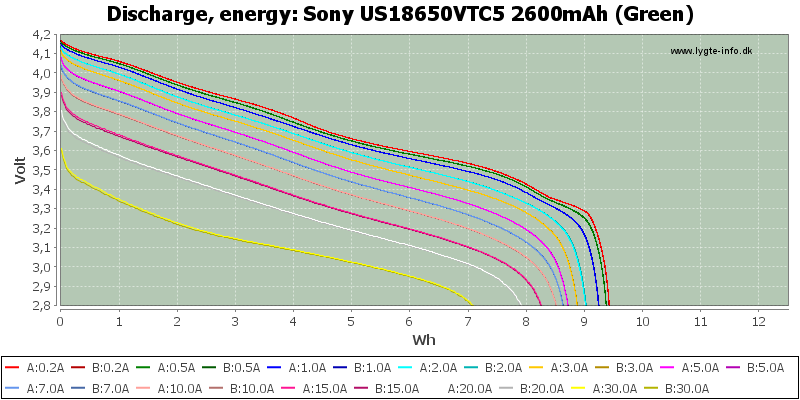
\includegraphics[scale=0.6]{pictures/vtc5.png}
	\caption{Discharge voltage vs. energy for Sony US18650VTC5 cells \cite{vtc5}}
	\label{fig:vtc5}
\end{figure}

\chapter{Balancing test}
\begin{figure}[h]
	\centering
	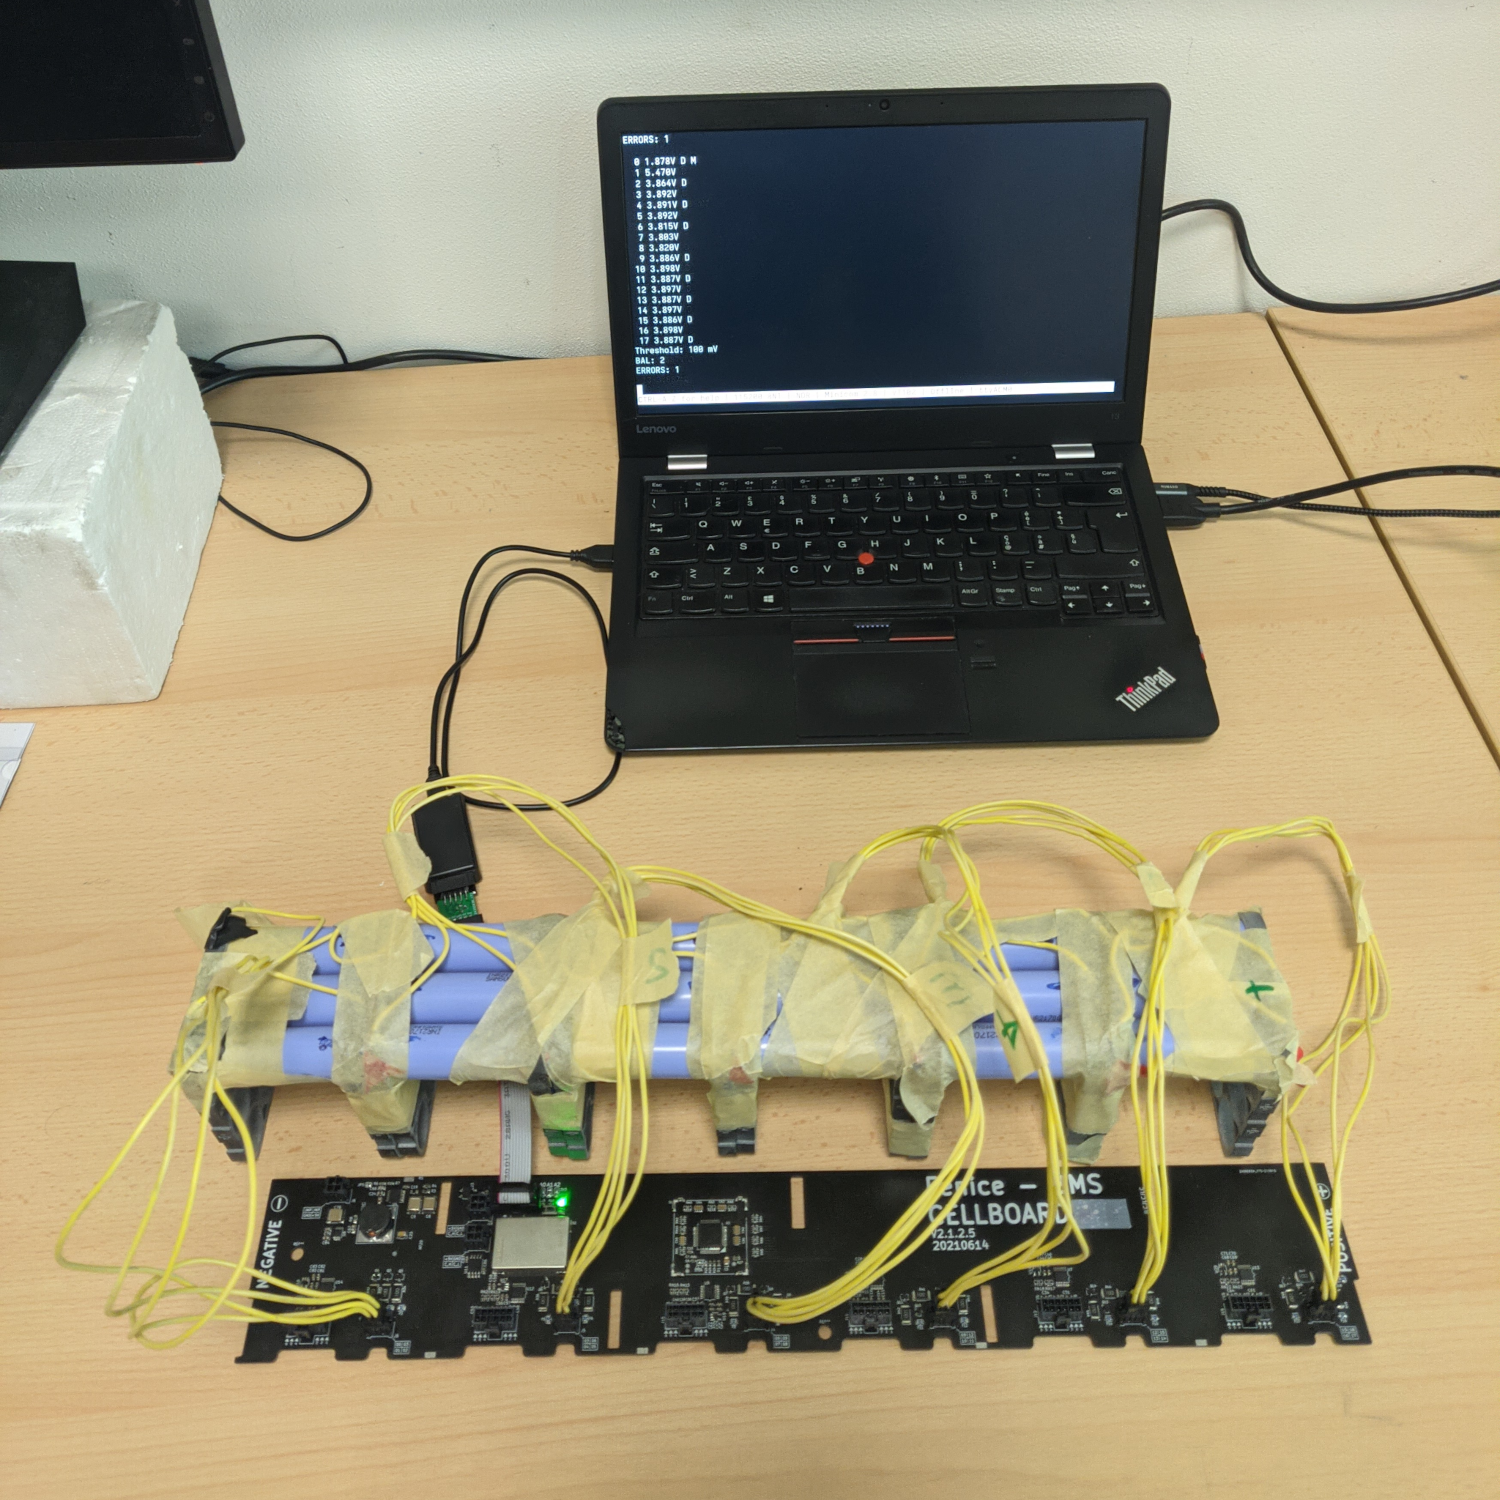
\includegraphics[scale=0.25]{balancing_test.png}
	\caption{Cell balancing test setup.}
	\label{fig:balancing_test}
\end{figure}
\begin{figure}[h]
	\centering
	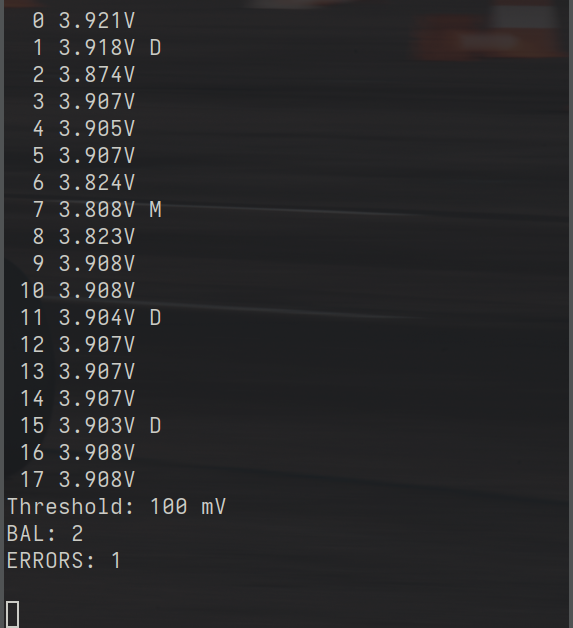
\includegraphics[scale=0.5]{balancing_console}
	\caption{Serial console during balancing. \texttt{M} indicates the minimum voltage, cells marked with \texttt{D} are being discharged}
	\label{fig:balancing_console}
\end{figure}

\chapter{Error management test}
\begin{figure}[h]
	\centering
	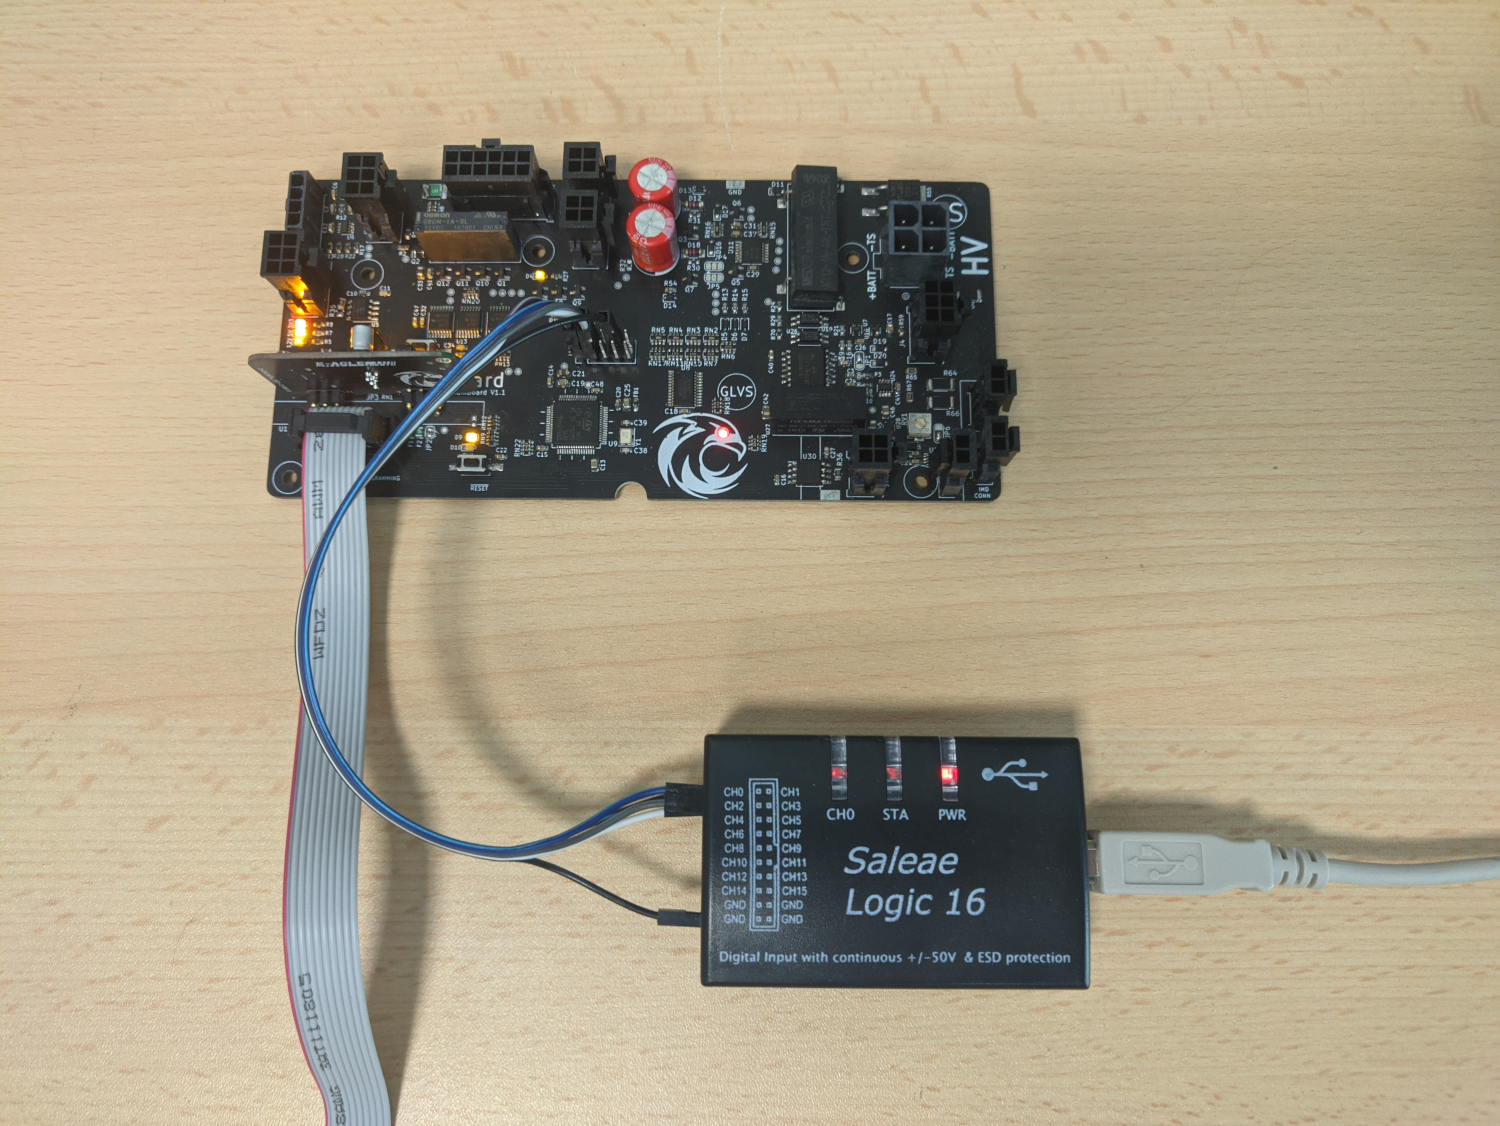
\includegraphics[scale=0.27]{error_test_setup.png}
	\caption{Error test setup with the mainboard and a logic analyzer.}
	\label{fig:error_test_setup}
\end{figure}
\begin{figure}[h]
	\centering
	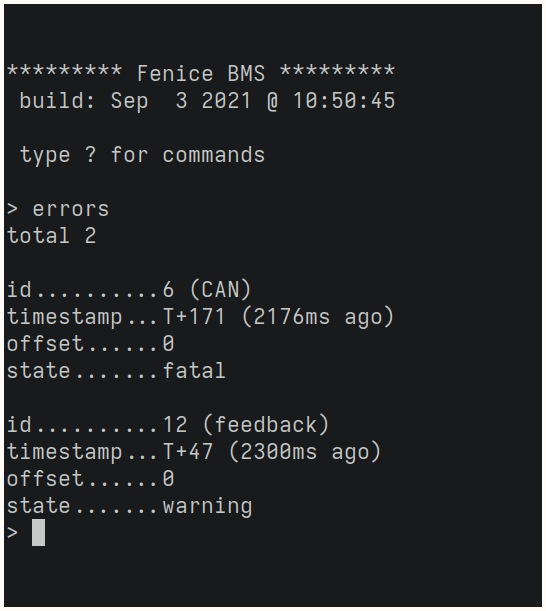
\includegraphics[scale=0.5]{error_console}
	\caption{Serial console reporting active errors.}
	\label{fig:error_console}
\end{figure}

\end{document}
